% ------------------------------------------------------------
% LaTeX Template für die DHBW zum Schnellstart!
% Original: https://github.wdf.sap.corp/vtgermany/LaTeX-Template-DHBW
% ------------------------------------------------------------
% ---- Präambel mit Angaben zum Dokument
\documentclass[
	fontsize=12pt,           % Leitlinien sprechen von Schriftgröße 12.
	paper=A4,
	twoside=false,
	listof=totoc,            % Tabellen- und Abbildungsverzeichnis ins Inhaltsverzeichnis
	bibliography=totoc,      % Literaturverzeichnis ins Inhaltsverzeichnis aufnehmen
	titlepage,               % Titlepage-Umgebung anstatt \maketitle
	headsepline,             % horizontale Linie unter Kolumnentitel
	abstract,              % Überschrift einschalten, Abstract muss in {abstract}-Umgebung stehen
]{scrreprt}                  % Verwendung von KOMA-Report
\usepackage[utf8]{inputenc}  % UTF8 Encoding einschalten
\usepackage[ngerman]{babel}  % Neue deutsche Rechtschreibung
\usepackage[T1]{fontenc}     % Ausgabe von westeuropäischen Zeichen (auch Umlaute)
\usepackage{microtype}       % Trennung von Wörtern wird besser umgesetzt
\usepackage{lmodern}         % Nicht-gerasterte Schriftarten (bei MikTeX erforderlich)
\usepackage{graphicx}        % Einbinden von Grafiken erlauben
\usepackage{wrapfig}         % Grafiken fließend im Text
\usepackage{setspace}        % Zeilenabstand \singlespacing, \onehalfspaceing, \doublespacing
\usepackage[
	%showframe,                % Ränder anzeigen lassen
	left=2.7cm, right=2.5cm,
	top=2.5cm,  bottom=2.5cm,
	includeheadfoot
]{geometry}                      % Seitenlayout einstellen
\usepackage{scrlayer-scrpage}    % Gestaltung von Fuß- und Kopfzeilen
\usepackage{acronym}             % Abkürzungen, Abkürzungsverzeichnis
\usepackage{titletoc}            % Anpassungen am Inhaltsverzeichnis
\contentsmargin{0.75cm}          % Abstand im Inhaltsverzeichnis zw. Punkt und Seitenzahl
\usepackage[                     % Klickbare Links (enth. auch "nameref", "url" Package)
  hidelinks,                     % Blende die "URL Boxen" aus.
  breaklinks=true                % Breche zu lange URLs am Zeilenende um
]{hyperref}
\usepackage[hypcap=true]{caption}% Anker Anpassung für Referenzen
\urlstyle{same}                  % Aktuelle Schrift auch für URLs
% Anpassung von autoref für Gleichungen (ergänzt runde Klammern) und Algorithm.
% Anstatt "Listing" kann auch z.B. "Code-Ausschnitt" verwendet werden. Dies sollte
% jedoch synchron gehalten werden mit \lstlistingname (siehe weiter unten).
\addto\extrasngerman{%
	\def\equationautorefname~#1\null{Gleichung~(#1)\null}
	\def\lstnumberautorefname{Zeile}
	\def\lstlistingautorefname{Listing}
	\def\algorithmautorefname{Algorithmus}
	% Damit einheitlich "Abschnitt 1.2[.3]" verwendet wird und nicht "Unterabschnitt 1.2.3"
	% \def\subsectionautorefname{Abschnitt}
}

% ---- Abstand verkleinern von der Überschrift 
\renewcommand*{\chapterheadstartvskip}{\vspace*{.5\baselineskip}}

% Hierdurch werden Schusterjungen und Hurenkinder vermieden, d.h. einzelne Wörter
% auf der nächsten Seite oder in einer einzigen Zeile.
% LaTeX kann diese dennoch erzeugen, falls das Layout ansonsten nicht umsetzbar ist.
% Diese Werte sind aber gute Startwerte.
\widowpenalty10000
\clubpenalty10000

% ---- Für das Quellenverzeichnis
\usepackage[
	backend = biber,                % Verweis auf biber
	language = auto,
	style = alphabetic,                % Nummerierung der Quellen mit Zahlen
	sorting = anyt,                 % none = Sortierung nach der Erscheinung im Dokument
	sortcites = true,               % Sortiert die Quellen innerhalb eines cite-Befehls
	block = space,                  % Extra Leerzeichen zwischen Blocks
	hyperref = true,                % Links sind klickbar auch in der Quelle
	%backref = true,                % Referenz, auf den Text an die zitierte Stelle
	bibencoding = auto,
	giveninits = true,              % Vornamen werden abgekürzt
	doi=false,                      % DOI nicht anzeigen
	isbn=false,                     % ISBN nicht anzeigen
    alldates=short                  % Datum immer als DD.MM.YYYY anzeigen
]{biblatex}
\addbibresource{Inhalt/literatur.bib}
\setcounter{biburlnumpenalty}{3000}     % Umbruchgrenze für Zahlen
\setcounter{biburlucpenalty}{6000}      % Umbruchgrenze für Großbuchstaben
\setcounter{biburllcpenalty}{9000}      % Umbruchgrenze für Kleinbuchstaben
\DeclareNameAlias{default}{family-given}  % Nachname vor dem Vornamen
\AtBeginBibliography{\renewcommand{\multinamedelim}{\addslash\space
}\renewcommand{\finalnamedelim}{\multinamedelim}}  % Schrägstrich zwischen den Autorennamen
\DefineBibliographyStrings{german}{
  urlseen = {Einsichtnahme:},                      % Ändern des Titels von "besucht am"
}
\usepackage[babel,german=quotes]{csquotes}         % Deutsche Anführungszeichen + Zitate


% ---- Für Mathevorlage
\usepackage{amsmath}    % Erweiterung vom Mathe-Satz
\usepackage{amssymb}    % Lädt amsfonts und weitere Symbole
\usepackage{MnSymbol}   % Für Symbole, die in amssymb nicht enthalten sind.


% ---- Für Quellcodevorlage
\usepackage{scrhack}                    % Hack zur Verw. von listings in KOMA-Script
\usepackage{listings}                   % Darstellung von Quellcode
\usepackage{xcolor}                     % Einfache Verwendung von Farben
% -- Eigene Farben für den Quellcode
\definecolor{JavaLila}{rgb}{0.4,0.1,0.4}
\definecolor{JavaGruen}{rgb}{0.3,0.5,0.4}
\definecolor{JavaBlau}{rgb}{0.0,0.0,1.0}
\definecolor{ABAPKeywordsBlue}{HTML}{6000ff}
\definecolor{ABAPCommentGrey}{HTML}{808080}
\definecolor{ABAPStringGreen}{HTML}{4da619}
\definecolor{PyKeywordsBlue}{HTML}{0000AC}
\definecolor{PyCommentGrey}{HTML}{808080}
\definecolor{PyStringGreen}{HTML}{008080}
% -- Farben für ABAP CDS
\definecolor{CDSString}{HTML}{FF8C00}
\definecolor{CDSKeywords}{HTML}{6000ff}
\definecolor{CDSAnnotation}{HTML}{00BFFF}
\definecolor{CDSComment}{HTML}{808080}
\definecolor{CDSFunc}{HTML}{FF0000}
% -- Farben für SQL
\definecolor{SQLString}{HTML}{15ABF6}
\definecolor{SQLKeywords}{HTML}{7B30FF}
\definecolor{SQLVariables}{HTML}{000000}

% -- Default Listing-Styles

\lstset{
	% Das Paket "listings" kann kein UTF-8. Deswegen werden hier 
	% die häufigsten Zeichen definiert (ä,ö,ü,...)
	literate=%
		{á}{{\'a}}1 {é}{{\'e}}1 {í}{{\'i}}1 {ó}{{\'o}}1 {ú}{{\'u}}1
		{Á}{{\'A}}1 {É}{{\'E}}1 {Í}{{\'I}}1 {Ó}{{\'O}}1 {Ú}{{\'U}}1
		{à}{{\`a}}1 {è}{{\`e}}1 {ì}{{\`i}}1 {ò}{{\`o}}1 {ù}{{\`u}}1
		{À}{{\`A}}1 {È}{{\'E}}1 {Ì}{{\`I}}1 {Ò}{{\`O}}1 {Ù}{{\`U}}1
		{ä}{{\"a}}1 {ë}{{\"e}}1 {ï}{{\"i}}1 {ö}{{\"o}}1 {ü}{{\"u}}1
		{Ä}{{\"A}}1 {Ë}{{\"E}}1 {Ï}{{\"I}}1 {Ö}{{\"O}}1 {Ü}{{\"U}}1
		{â}{{\^a}}1 {ê}{{\^e}}1 {î}{{\^i}}1 {ô}{{\^o}}1 {û}{{\^u}}1
		{Â}{{\^A}}1 {Ê}{{\^E}}1 {Î}{{\^I}}1 {Ô}{{\^O}}1 {Û}{{\^U}}1
		{œ}{{\oe}}1 {Œ}{{\OE}}1 {æ}{{\ae}}1 {Æ}{{\AE}}1 {ß}{{\ss}}1
		{ű}{{\H{u}}}1 {Ű}{{\H{U}}}1 {ő}{{\H{o}}}1 {Ő}{{\H{O}}}1
		{ç}{{\c c}}1 {Ç}{{\c C}}1 {ø}{{\o}}1 {å}{{\r a}}1 {Å}{{\r A}}1
		{€}{{\euro}}1 {£}{{\pounds}}1 {«}{{\guillemotleft}}1
		{»}{{\guillemotright}}1 {ñ}{{\~n}}1 {Ñ}{{\~N}}1 {¿}{{?`}}1,
	breaklines=true,        % Breche lange Zeilen um 
	breakatwhitespace=true, % Wenn möglich, bei Leerzeichen umbrechen
	% Symbol für Zeilenumbruch einfügen
	prebreak=\raisebox{0ex}[0ex][0ex]{\ensuremath{\rhookswarrow}},
	postbreak=\raisebox{0ex}[0ex][0ex]{\ensuremath{\rcurvearrowse\space}},
	tabsize=4,                                 % Setze die Breite eines Tabs
	basicstyle=\ttfamily\small,                % Grundsätzlicher Schriftstyle
	columns=fixed,                             % Besseres Schriftbild
	numbers=left,                              % Nummerierung der Zeilen
	%frame=single,                             % Umrandung des Codes
	showstringspaces=false,                    % Keine Leerzeichen hervorheben
	keywordstyle=\color{blue},
	ndkeywordstyle=\bfseries\color{darkgray},
	identifierstyle=\color{black},
	commentstyle=\itshape\color{JavaGruen},   % Kommentare in eigener Farbe
	stringstyle=\color{JavaBlau},             % Strings in eigener Farbe,
	captionpos=b,                             % Bild*unter*schrift
	xleftmargin=5.0ex
}

% ---- Eigener JAVA-Style für den Quellcode
\renewcommand{\ttdefault}{pcr}               % Schriftart, welche auch fett beinhaltet
\lstdefinestyle{EigenerJavaStyle}{
	language=Java,                             % Syntax Highlighting für Java
	%frame=single,                             % Umrandung des Codes
	keywordstyle=\bfseries\color{JavaLila},    % Keywords in eigener Farbe und fett
	commentstyle=\itshape\color{JavaGruen},    % Kommentare in eigener Farbe und italic
	stringstyle=\color{JavaBlau}               % Strings in eigener Farbe
}

% ---- Eigener ABAP-Style für den Quellcode
\renewcommand{\ttdefault}{pcr}
\lstdefinestyle{EigenerABAPStyle}{
	language=[R/3 6.10]ABAP,
	morestring=[b]\|,                          % Für Pipe-Strings
	morestring=[b]\`,                          % für Backtick-Strings
	keywordstyle=\bfseries\color{ABAPKeywordsBlue},
	commentstyle=\itshape\color{ABAPCommentGrey},
	stringstyle=\color{ABAPStringGreen},
	tabsize=2,
	morekeywords={
		types,
		@data,
		as,
		lower,
		start,
		selection,
		order,
		by,
		inner,
		join,
		key,
		end,
		cast
	}
}

% ---- Eigener SQL-Style für den Quellcode
\renewcommand{\ttdefault}{pcr}
\lstdefinestyle{EigenerSQLStyle}{
	language=SQL,
	keywordstyle=\bfseries\color{SQLKeywords},
	commentstyle=\itshape\color{ABAPCommentGrey},
	stringstyle=\color{SQLString},
	morekeywords={
		SELECT,
		INSERT,
		CREATE,
		UPDATE,
		MOVE,
		AS,
		ON,
		COUNT,
		MAX,
		MIN,
		DELETE,
		GRANT,
		PERMISSIONS,
		ALL,
		REVOKE,
		INNER JOIN,
		RIGHT JOIN,
		LEFT JOIN,
		FULL JOIN,
		FULL OUTER JOIN,
		CROSS JOIN,
		IS,
		NULL,
		DISTINCT,
		JOIN
	}
}

% ---- Eigener Python-Style für den Quellcode
\renewcommand{\ttdefault}{pcr}
\lstdefinestyle{EigenerPythonStyle}{
	language=Python,
	columns=flexible,
	keywordstyle=\bfseries\color{PyKeywordsBlue},
	commentstyle=\itshape\color{PyCommentGrey},
	stringstyle=\color{PyStringGreen}
}

%----- ABAP-CDS-View language
\lstdefinelanguage{ABAPCDS}{
	sensitive=false,
	%Keywords
	morekeywords={define,
		view,
		as,
		select,
		from,
		inner,
		join,
		on,
		key,
		case,
		when,
		then,
		else,
		end,
		true,
		false,
		cast,
		where,
		and,
		distinct,
		group,
		by,
		having,
		min,
		sum,
		max,
		count,
		avg
	},
	%Methoden
	morekeywords=[2]{
		div,
		currency\_conversion,
		dats\_days\_between,
		concat\_with\_space,
		dats\_add_days,
		dats\_is\_valid,
		dats\_add\_months,
		unit\_conversion,
		division,
		mod,
		abs,
		floor,
		ceil,
		round,
		concat,
		replace,
		substring,
		left,
		right,
		length
	},
	morecomment=[s][\color{CDSAnnotation}]{@}{:},
	morecomment=[l][\itshape\color{CDSComment}]{//},
	morecomment=[s][\itshape\color{CDSComment}]{/*}{*/},
	morestring=[b][\color{CDSString}]',
	keywordstyle=\bfseries\color{CDSKeywords},
	keywordstyle=[2]\color{CDSFunc}
}

  % Weitere Details sind ausgelagert

\usepackage{algorithm}                  % Für Algorithmen-Umgebung (ähnlich wie lstlistings Umgebung)
\usepackage{algpseudocode}              % Für Pseudocode. Füge "[noend]" hinzu, wenn du kein "endif",
                                        % etc. haben willst.

\makeatletter                           % Sorgt dafür, dass man @ in Namen verwenden kann.
                                        % Ansonsten gibt es in der nächsten Zeile einen Compilefehler.
\renewcommand{\ALG@name}{Algorithmus}   % Umbenennen von "Algorithm" im Header der Listings.
\makeatother                            % Zeichen wieder zurücksetzen
\renewcommand{\lstlistingname}{Code} % Erlaubt das Umbenennen von "Listing" in anderen Titel.

% ---- Tabellen
\usepackage{booktabs}  % Für schönere Tabellen. Enthält neue Befehle wie \midrule
\usepackage{multirow}  % Mehrzeilige Tabellen
\usepackage{siunitx}   % Für SI Einheiten und das Ausrichten Nachkommastellen
\sisetup{locale=DE, range-phrase={~bis~}, output-decimal-marker={,}} % Damit ein Komma und kein Punkt verwendet wird.
\usepackage{xfrac} % Für siunitx Option "fraction-function=\sfrac"

% ---- Für Definitionsboxen in der Einleitung
\usepackage{amsthm}                     % Liefert die Grundlagen für Theoreme
\usepackage[framemethod=tikz]{mdframed} % Boxen für die Umrandung
% ---- Definition für Highlight Boxen

% ---- Grundsätzliche Definition zum Style
\newtheoremstyle{defi}
  {\topsep}         % Abstand oben
  {\topsep}         % Abstand unten
  {\normalfont}     % Schrift des Bodys
  {0pt}             % Einschub der ersten Zeile
  {\bfseries}       % Darstellung von der Schrift in der Überschrift
  {:}               % Trennzeichen zwischen Überschrift und Body
  {.5em}            % Abstand nach dem Trennzeichen zum Body Text
  {\thmname{#3}}    % Name in eckigen Klammern
\theoremstyle{defi}

% ------ Definition zum Strich vor eines Texts
\newmdtheoremenv[
  hidealllines = true,       % Rahmen komplett ausblenden
  leftline = true,           % Linie links einschalten
  innertopmargin = 0pt,      % Abstand oben
  innerbottommargin = 4pt,   % Abstand unten
  innerrightmargin = 0pt,    % Abstand rechts
  linewidth = 3pt,           % Linienbreite
  linecolor = gray!40,       % Linienfarbe
]{defStrich}{Definition}     % Name der des formats "defStrich"

% ------ Definition zum Eck-Kasten um einen Text
\newmdtheoremenv[
  hidealllines = true,
  innertopmargin = 6pt,
  linecolor = gray!40,
  singleextra={              % Eck-Markierungen für die Definition
    \draw[line width=3pt,gray!50,line cap=rect] (O|-P) -- +(1cm,0pt);
    \draw[line width=3pt,gray!50,line cap=rect] (O|-P) -- +(0pt,-1cm);
    \draw[line width=3pt,gray!50,line cap=rect] (O-|P) -- +(-1cm,0pt);
    \draw[line width=3pt,gray!50,line cap=rect] (O-|P) -- +(0pt,1cm);
  }
]{defEckKasten}{Definition}  % Name der des formats "defEckKasten"  % Weitere Details sind ausgelagert

% ---- Für Todo Notes
\usepackage{todonotes}
\setlength {\marginparwidth }{2cm}      % Abstand für Todo Notizen

\usepackage{pdfpages}
\usepackage{jslistings}

% ---- Elektronische Version oder Gedruckte Version?
% ---- Unterschied: Die elektronische Version enthält keinen Platzhalter für die Unterschrift
\usepackage{ifthen}
\newboolean{e-Abgabe}
\setboolean{e-Abgabe}{true}    % false=gedruckte Fassung

% ---- Persönlichen Daten:
\newcommand{\titel}{High-Level Vergleich von Big Data Dateiformaten}
\newcommand{\titelheader}{Integrationsseminar}
\newcommand{\arbeit}{Seminararbeit}
\newcommand{\studiengang}{Wirtschaftsinformatik: Software Engineering}
\newcommand{\studienjahr}{2022}
\newcommand{\autor}{Mathis Neunzig}
\newcommand{\autorReverse}{Neunzig, Mathis}
\newcommand{\verfassungsort}{Mannheim}
\newcommand{\matrikelnr}{2240587}
\newcommand{\kurs}{WI 2020 MA SE B}
\newcommand{\bearbeitungsmonat}{Dezember 2022 - Februar 2023}
\newcommand{\abgabe}{03. Februar 2023}
\newcommand{\bearbeitungszeitraum}{22.12.2022 - 03.02.2023}
\newcommand{\dozent}{Alexander Lütke}
\newcommand{\firmaName}{SAP SE}
\newcommand{\firmaStrasse}{Dietmar-Hopp-Allee 16}
\newcommand{\firmaPlz}{69190 Walldorf, Deutschland}
\newcommand{\betreuerFirma}{Joscha-Philipp Bohn}
\newcommand{\betreuerDhbw}{Prof. Dr. Thomas Holey}

% ---- Adressen:
\newcommand{\sapdeName}{SAP Deutschland SE und Co. KG}
\newcommand{\sapdeStrasse}{Hasso-Plattner-Ring 7}
\newcommand{\sapdePLZ}{69190 Walldorf, Deutschland}
\newcommand{\aribaName}{Ariba Inc. (SAP Ariba)}
\newcommand{\aribaStrasse}{3420 Hillview Ave}
\newcommand{\aribaPLZ}{CA 94304 Palo Alto, USA}
\newcommand{\concurName}{Concur Technologies Inc., Concur Holdings (Netherlands) B.V. (SAP Concur)}
\newcommand{\concurStrasse}{601 108th Ave NE}
\newcommand{\concurPLZ}{WA 98004 Bellevue, USA}
\newcommand{\fgName}{SAP America Inc., SAP Fieldglass, SAP SuccessFactors}
\newcommand{\fgStrasse}{3999 West Chester Pike}
\newcommand{\fgPLZ}{PA 19073 Newtown Square, USA}
\newcommand{\hybrisName}{hybris AG (SAP Hybris)}
\newcommand{\hybrisStrasse}{Birkenstrasse 49}
\newcommand{\hybrisPLZ}{6343 Rotkreuz, Schweiz}
\newcommand{\gName}{Gartner Inc.}
\newcommand{\gStrasse}{56 Top Gallant Road}
\newcommand{\gPLZ}{Stamford, CT 06902 USA}

% ---- Metainformation für das PDF Dokument
\hypersetup{
	pdftitle    = {\titel},
	pdfsubject  = {\arbeit},
	pdfauthor   = {\autor},
	%pdfkeywords = {Keywords angeben},
	pdfcreator  = {LaTeX},
	%pdfproducer = {in der Regel pdfTeX}
}

% ---- Definition der Kopf- und Fußzeilen
\clearpairofpagestyles                          % Löschen von LaTeX Standard
\automark[section]{chapter}                     % Füllen von section und chapter
\renewcommand*{\chaptermarkformat}{}            % Entfernt die Kapitelnummer
\renewcommand*{\sectionmarkformat}{}            % Entfernt die Sectionnummer
% Angaben [für "plain"]{für "scrheadings"}
\ihead[]{\titelheader}                          % Kopfzeile links
\chead[]{}                                      % Kopfzeile mitte
\ohead[]{\rightmark}                            % Kopfzeile rechts
\ifoot[]{}                                      % Fußzeile links
\cfoot*{\sffamily\pagemark}                     % Fußzeile mitte
\ofoot[]{}                                      % Fußzeile rechts
\KOMAoptions{
   headsepline = 0.2pt,                         % Liniendicke Kopfzeile
   footsepline = false                          % Liniendicke Fußzeile
}


% ---- Hilfreiches
\newcommand{\zB}{z.\,B. }   % "z.B." mit kleinem Leeraum dazwischen (ohne wäre nicht korrekt)
\newcommand{\dash}{d.\,h. }

\newcommand{\code}[1]{\texttt{#1}} % Ist einfacher zu schreiben als ständig \texttt und erlaubt
                                   % Änderungen im Nachhinein, wenn man z.B. Inline-Code anders stylen möchte.

% ---- Silbentrennung (falls LaTeX defaults falsch / nicht gewünscht sind)
\hyphenation{HANA}         % anstatt HA-NA
\hyphenation{Graph-Script} % anstatt GraphS-cript

% ---- Beginn des Dokuments
\begin{document}
\setlength{\parindent}{0pt}              % Keine Paragraphen Einrückung.
                                         % Dafür haben wir den Abstand zwischen den Paragraphen.
\setcounter{secnumdepth}{2}              % Nummerierungstiefe fürs Inhaltsverzeichnis
\setcounter{tocdepth}{2}                 % Tiefe des Inhaltsverzeichnisses. Ggf. so anpassen,
                                         % dass das Verzeichnis auf eine Seite passt.
\sffamily                                % Serifenlose Schrift verwenden.

% ---- Vorspann
% ------ Titelseite
\singlespacing
\thispagestyle{empty}
\begin{titlepage}
\enlargethispage{4cm}

\begin{figure}           % Logo vom Ausbildungsbetrieb und der DHBW
	\vspace*{-5mm} % Sollte dein Titel zu lang werden, kannst du mit diesem "Hack" 
	%                  den Inhalt der Seite nach oben schieben.
	%\begin{minipage}{0.49\textwidth}
	%	\flushleft
	%	\includegraphics[height=2.5cm]{Bilder/Logos/Logo_SAP.pdf} 
	%\end{minipage}
	\begin{minipage}{0.49\textwidth}
		\flushleft
		
\includegraphics[height=2.5cm]{Bilder/Logos/Logo_DHBW.pdf} 
	\end{minipage}
\end{figure} 
\vspace*{0.1cm}

\begin{center}
	\huge{\textbf{\titel}}\\[1.5cm]
	\Large{\textbf{\arbeit}}\\[0.5cm]
	\normalsize{im Rahmen der Prüfung zum\\[1ex] \textbf{Bachelor of Science (B.Sc.)}}\\[0.5cm]
	\Large{des Studienganges \studiengang}\\[1ex]
	\normalsize{an der Dualen Hochschule Baden-Württemberg Mannheim}\\[1cm]
	\normalsize{von}\\[1ex] \Large{\textbf{\autor}} \\[1cm]
	% Hinweis: Manche Dozenten möchten einen Hinweis auf den Sperrvermerk auf der Titelseite.
	% \large{{\color{red}- Sperrvermerk -}}\\[1cm]
\end{center}

\begin{center}
	\begin{tabular}{ll}
		Abgabedatum:                     & \abgabe \\[0.2cm]
		Bearbeitungszeitraum:            & \bearbeitungszeitraum \\[0.2cm]
		Matrikelnummer, Kurs:            & \matrikelnr , \kurs \\[0.2cm]
		Ausbildungsfirma:                & \firmaName \\
		                                 & \firmaStrasse \\
		                                 & \firmaPlz \\[0.2cm]
		Betreuender Dozent:   & \dozent \\[0.2cm]
	\end{tabular} 
\end{center}
\end{titlepage}
  % Titelseite
\newcounter{savepage}
\pagenumbering{Roman}                    % Römische Seitenzahlen
\onehalfspacing

% ------ Erklärung, Sperrvermerk, Abstact, Vorwort
\chapter*{Eidesstattliche Erklärung}
Ich versichere hiermit, dass ich meine \arbeit{} mit dem Thema:
\begin{quote}
	\textit{\titel}
\end{quote} 
gemäß § 5 (4) der \enquote{StuPrO DHBW Wirtschaft 2018} vom 11. Oktober 2018 mit der vierten Änderung vom 14. Juli 2022 selbstständig verfasst und keine anderen als die angegebenen Quellen und Hilfsmittel benutzt habe. Die Arbeit wurde bisher keiner anderen Prüfungsbehörde vorgelegt und auch nicht veröffentlicht.

\vspace{0.25cm}

Ich versichere zudem, dass die eingereichte elektronische Fassung mit der gedruckten Fassung übereinstimmt.

\vspace{1cm}

\verfassungsort, den \today \\[0.5cm]
\ifthenelse{\boolean{e-Abgabe}}
	{\underline{Gez. \autor}}
	{\makebox[6cm]{\hrulefill}}\\ 
\autorReverse

\renewcommand{\abstractname}{Abstract} % Veränderter Name für das Abstract
\begin{abstract}
\begin{addmargin}[1.5cm]{1.5cm}        % Erhöhte Ränder, für Abstract Look
\thispagestyle{plain}                  % Seitenzahl auf der Abstract Seite

\begin{center}
\small\textit{Mathis Neunzig - 2240587}             % Angabe der Sprache für das Abstract
\end{center}

\begin{center}
\small\textit{- Deutsch -}             % Angabe der Sprache für das Abstract
\end{center}

\vspace{0.25cm}
Das Thema Big Data wird in der globalisierten und modernen Welt immer wichtiger. Dadurch wachsen global die von Unternehmen, Privatpersonen und Organisationen gesammelten Daten auf unvorstellbare Größen an, die es mit Software zu verarbeiten gilt. Für die Verarbeitung solcher Daten sind spezielle Dateiformate erforderlich, die auf solche Zwecke ausgerichtet sind. 

\vspace{0.25cm}
Die Arbeit beschäftigt sich mit der Frage, in welchen Punkten sich gängige Big-Data-Dateiformate voneinander unterscheiden und wann welche eingesetzt werden sollen. Dabei werden verschiedene Dateiformate miteinander verglichen. Diese Dateiformate sind entweder in der Literatur als ''Big-Data-Dateiformate'' gekennzeichnet oder sind im Alltag im Einsatz und könnten für große Daten theoretisch benutzt werden. 

\vspace{0.25cm}
Die Dateiformate Parquet, Avro und ORC heben sich deutlich von Formaten wie CSV, JSON und XML ab, da diese kleiner, schneller und performanter sind. Parquet, Avro und ORC unterscheiden sich untereinander in einigen Punkten, weshalb für den konkreten Einsatz ein Dateiformat nach Analyse und Vergleichen ausgewählt werden sollte. 

\end{addmargin}
\end{abstract}
\chapter*{Disclaimer}
In dieser Arbeit wird aus Gründen der besseren Lesbarkeit auf die gleichzeitige Verwendung der Sprachformen männlich, weiblich und divers (m/w/d) verzichtet und das generische Maskulinum verwendet. Weibliche und anderweitige Geschlechteridentitäten werden dabei ausdrücklich mitgemeint, soweit es für die Aussage erforderlich ist.

\vspace{0.25cm}
Abbildungen und Codebeispiele befinden sich auf Grund von Größe oder Störung im Lesefluss im Anhang und nicht im laufenden Text. Sie tragen zur Unterscheidung eine laufende Nummer, die mit einem Buchstaben beginnt.

\vspace{0.25cm}
Literaturangaben sind mit eckigen Klammern gekenntzeichnet, in denen die Initialen oder die ersten Buchstaben der Autoren sowie, wenn vorhanden, das Jahr enthalten sind. Die kompletten Angaben zu diesen Materialien befinden sich alphabetisch sortiert im Literaturverzeichnis.

% ------ Inhaltsverzeichnis
\singlespacing
\tableofcontents

% ------ Verzeichnisse
\renewcommand*{\chapterpagestyle}{plain}
\pagestyle{plain}
\chapter*{Abkürzungsverzeichnis}
\addcontentsline{toc}{chapter}{Abkürzungsverzeichnis} % Hinzufügen zum Inhaltsverzeichnis 

\begin{acronym}[WYSISWG] % längstes Kürzel wird verw. für den Abstand zw. Kürzel u. Text

	% Alphabetisch selbst sortieren - nicht verwendete Kürzel rausnehmen!
	\acro{JSON}{JavaScript Object Notation}
    \acro{XML}{eXtensible Markup Language}
    \acro{CSV}{Comma Separated Values}
    \acro{ORC}{Optimized Row Columnar}

\end{acronym}
\listoffigures                          % Erzeugen des Abbildungsverzeichnisses 
\renewcommand{\lstlistlistingname}{Quellcodeverzeichnis}
\lstlistoflistings                      % Erzeugen des Listenverzeichnisses
\setcounter{savepage}{\value{page}}


% ---- Inhalt der Arbeit
\cleardoublepage
\pagenumbering{arabic}                  % Arabische Seitenzahlen für den Hauptteil
\setlength{\parskip}{0.5\baselineskip}  % Abstand zwischen Absätzen
\rmfamily
\renewcommand*{\chapterpagestyle}{scrheadings}
\pagestyle{scrheadings}
\onehalfspacing
\chapter{Einleitung}
Diese Seminararbeit ist im Zuge des Moduls ''Integrationsseminar'' entstanden, welches sich mit ausgewählten Aspekten der Wirtschaftsinformatik beschäftigt. Diese Arbeit speziell vergleicht wichtige Big-Data-Dateiformate miteinander.

Mit dem Voranschreiten der digitalen Transformation und der Globalisierung wird das Thema Big Data immer wichtiger. Dadurch, dass in den verschiedensten Bereichen der Wirtschaft immer mehr Daten gebraucht werden, müssen diese Daten effizient und schnell verarbeitet werden \cite{verbraucherzentralede_geschichte_nodate}. Dabei steht ''Big Data'' für die große Datenmenge, die menschlich nicht erfassbar ist und moderne Entscheidungsmechanismen übernimmt \cite{sap_was_nodate}. 

Zu Beginn werden die Dateiformate vorgestellt, bevor Aufgrund von bestimmten Kriterien eine Auswahl getroffen wird, welche Dateiformate als Big-Data-Dateiformate klassifiziert werden könnten und somit verglichen werden. Diese werden im Anschluss miteinander im Bezug auf verschiedene Charakteristiken, die im weiteren Verlauf erläutert werden, untersucht und verglichen. Die Daten und Fakten, auf denen die Vergleiche basieren, stammen aus einer breit gefächerten Literaturrecherche zu den einzelnen Dateiformaten, sowie Verbindungen und Vergleiche zwischen diesen. 

\chapter{Theoretische Grundlagen}

\section{Apache Parquet}
Parquet ist ein nicht von Menschen lesbares, codiertes Datei-Format für die Speicherung von Big Data und ist in der Lage, große Mengen an Daten zu speichern und diese wieder schnell zu lesen \cite{apache_apache_nodate} \cite[S. 906]{gohil_compendious_2022}. Es ordnet die Daten in Spalten, was die Lesezeit erheblich reduzieren und die Performance verbessern kann\footnote{Siehe Abbildung \ref{fig:Parquet}} \cite[S. 339]{munir_cost-based_2020}. Ein exemplarischer Aufbau ist in Anhang in der Abbildung \ref{fig:Parquet} zu finden. Es unterstützt auch fortgeschrittene Funktionen wie Prädikat-Pushdown, bei dem nur die relevanten Daten gelesen werden und Datenkomprimierung, um die Größe der Daten zu minimieren \cite[S. 268]{plase_comparison_2017}. Es verwendet ein festes Schema, was bedeutet, dass die Struktur der Daten vorab definiert ist und sich nicht mehr ändern kann. Dies hilft in der Optimierung der Performance und der Datenverwaltung \cite{apache_apache_nodate}.

\section{Apache Avro}
Apache Avro ist ein Datenserialisierungsformat, das entwickelt wurde, um Daten effizient zu serialisieren, zu deserialisieren und zu verarbeiten \cite{apache_avro_nodate}. Die Daten in Avro-Dateien sind, ähnlich wie bei CSV, reihenweise abgespeichert\footnote{Siehe Abbildung \ref{fig:Avro}}, kann jedoch durch die Codierung des Inhalts wie bei Parquet nicht von Menschen gelesen werden \cite[S. 338]{munir_cost-based_2020} \cite[S. 906]{gohil_compendious_2022}. Ein exemplarischer Aufbau einer Avro-Datei ist im Anhang in der Abbildung \ref{fig:Avro} zu finden. Avro verwendet ein festes Schema, um die Datenstruktur und -integrität sicherzustellen. Das Schema wird in der Datei selbst gespeichert, was es ermöglicht, die Daten ohne Kenntnis des Schemas zu lesen und zu verarbeiten. Avro unterstützt auch die Datenkompression, um die Datengröße zu reduzieren und die Übertragungszeit zu verkürzen \cite[S. 268]{plase_comparison_2017}. Es ist für die Verwendung mit Big-Data-Verarbeitungsrahmen wie Apache Kafka optimiert \cite[S. 906]{gohil_compendious_2022}.

\section{ORC}
Apache \ac{ORC} speichert Daten in einer spaltenorientierten Weise\footnote{Siehe Abbildung \ref{fig:ORC}}, wodurch es gezielt nur die benötigten Spalten lesen und verarbeiten kann, anstatt die gesamte Datenzeile \cite[S. 339]{munir_cost-based_2020} \cite{apache_languagemanual_nodate} \cite[S. 906]{gohil_compendious_2022}. Wie Avro und Parquet ist ORC codiert und in roher Form nicht von Menschen lesbar. Ein exemplarischer Aufbau kann in Anhang in der Abbildung \ref{fig:ORC} gefunden werden. Durch den Aufbau kann die Lesezeit erheblich reduzieren und die Performance verbessert werden. Es unterstützt Datenkomprimierung, um die Größe der Daten zu minimieren \cite[S. 268]{plase_comparison_2017}. ORC ist ein Dateiformat für den Einsatz mit Big-Data-Verarbeitungsrahmen wie Apache Hive. 

\section{Sonstige Dateiformate}
\subsubsection{XML}
\ac{XML} ist ein von Menschen lesbares, standardisiertes Format zur Beschreibung und Übertragung von Daten. Es basiert auf einer hierarchischen Struktur von Tags (Markups) und Attributen, die die Bedeutung und Struktur der Daten beschreiben\footnote{Siehe Codebeispiel \ref{code:XML}}. XML ermöglicht es Entwicklern, eigene Tags und Attribute zu definieren, um die Daten passgenau beschreiben zu können \cite[S. 7ff.]{nolan_xml_2014} \cite[S. 906]{gohil_compendious_2022}.

\subsubsection{JSON}
\ac{JSON} ist ein standardisiertes Format für die Übertragung und Speicherung von Daten, welches wie XML auch von Menschen lesbar ist. Es basiert auf der Syntax von JavaScript und verwendet eine klare, textbasierte Notation, um Daten in einer Hierarchie von Schlüssel-Wert-Paaren darzustellen\footnote{Siehe Codebeispiel \ref{code:JSON}} \cite[S. 4]{belov_experimental_2021} \cite[S. 14ff.]{nolan_xml_2014} \cite[S. 906]{gohil_compendious_2022}.

\subsubsection{CSV}
\ac{CSV} ist ein einfaches Textdatei-Format zur Speicherung von Tabellendaten. Die Daten werden in Form von Zeilen und Spalten gespeichert, wobei die Spalten durch Kommas voneinander getrennt sind\footnote{Siehe Codebeispiel \ref{code:CSV}}. Jede Zeile entspricht einer Datenzeile, wobei die erste Zeile den Namen der Spalten enthalten kann \cite[S. 905]{gohil_compendious_2022}.

\chapter{Vergleiche}

In der Wissenschaft gibt es keine Einigkeit, welche Dateiformate als ''Big-Data-Dateiformate'' eingestuft werden können. Es gibt Literatur, die eine Vielzahl von Dateiformaten in den Bereich einordnet und diese miteinander vergleicht \cite{gohil_compendious_2022} \cite{belov_experimental_2021} \cite{belov_analysis_2021}, jedoch gibt es auch solche Literatur, die nur Parquet, Avro und ORC als ''Big-Data-Dateiformate'' ansehen \cite{plase_comparison_2017}. Da Parquet, Avro und ORC auf den ersten Blick schnellere und kleinere Dateiformate sind \cite[S. 907ff.]{gohil_compendious_2022} \cite[S. 7]{belov_experimental_2021}, die sich somit mehr für ''Big Data'' eignen, werden nur diese drei Dateiformate in den folgenden Vergleichen herangezogen. Die übrigen Dateiformate JSON, CSV und XML werden nur sporadisch an kritischen Stellen erwähnt, wo dies nötig ist.

Nachdem die zu vergleichenden Dateiformate feststehen, können diese im Folgenden gegenübergestellt werden. In der Literatur werden oft die Metriken Speicherplatz, Geschwindigkeit und die Komprimierung von Dateiformaten untersucht. Deshalb werden diese Metriken neben anderen, seltener in der Literatur auftauchenden Metriken, im Folgenden untersucht. Für die Analyse werden Beispieldaten genutzt, welche aus einer Millionen Zeilen bestehen\footnote{Aufbau der Beispieldaten in \ref{fig:Daten}}.

Die untersuchten Dateiformate sind primär Parquet, Avro und ORC. Zusätzlich werden ein paar Vergleiche mit herkömmlichen Dateiformaten wie JSON, CSV und XML hergestellt.

\section{Speicherplatz}
Im Vergleich zu von Menschen lesbaren Dateiformaten wie JSON oder XML, werden Parquet, Avro und ORC codiert und sind nicht von Menschen lesbar \cite[S. 905f.]{gohil_compendious_2022}. Aus diesem Grund entfällt einiges an Overhead, wie zum Beispiel die Tags in XML oder die sich wiederholenden Attributbezeichnungen in JSON, welche den Speicherplatz sehr erhöhen. Aus diesem Grund sind Parquet-, Avro- und ORC-Dateien generell klein, jedoch ist Avro im Vergleich zu Parquet und ORC um einiges Größer und kann sogar mit dem zu den nicht-Big-Data-Dateiformaten gehörenden CSV verglichen werden\footnote{Siehe Abbildung \ref{fig:Speicherplatz}} \cite[S. 907]{gohil_compendious_2022} \cite[S. 7]{belov_experimental_2021}. Zu beachten ist, dass in Avro-Dateien das Schema im Klartext als JSON-Object mitgespeichert ist \cite[S. 338]{munir_cost-based_2020}.

\section{Geschwindigkeit}
Bei verschiedenen Lese-Zugriffen auf den Datensatz mit verschiedenen Funktionen stellt sich heraus, dass Avro um ein Vielfaches langsamer ist als ORC und Parquet \cite[S. 908ff.]{gohil_compendious_2022}. Dabei ist es egal, ob zufällige Daten gewählt werden\footnote{Siehe Abbildung \ref{fig:Zufall}}, Aggregationen ausgeführt werden\footnote{Siehe Abbildung \ref{fig:Aggregation}} oder mathematische Funktionen mit numerischen Spalten durchgeführt werden\footnote{Siehe Abbildung \ref{fig:Summierungen}}.
Da Avro eine zeilenweise Speicherung besitzt, können Daten schnell geschrieben werden. Das Lesen ist dentsprechend langsamer als die spaltenorientierten Formate Parquet und ORC, die widerum beim Schreiben in Dateien langsamer sind \cite[S. 1665]{abadi_column-oriented_nodate}. Bei allen Anfragen waren JSON, CSV und XML langsamer und nicht mit Parquet, Avro und ORC vergleichbar \cite[S. 906ff.]{gohil_compendious_2022}.

\section{Komprimierung}
Parquet, Avro als auch ORC unterstützen verschiedene Arten von Komprimierung \cite[S. 268]{plase_comparison_2017}, welches herkömmliche Dateiformate meist nicht anbieten \cite[S. 553]{belov_analysis_2021}. Parquet und ORC unterstützen beide eine Vielzahl von gleichen Komprimierungsarten, wie Snappy, LZ4 oder ZSTD. Avro unterstützt eine andere Menge an Komprimierungen, wie Deflate, BZIP2, XZ aber auch Snappy und ZSTD, wie Parquet und ORC auch. Die Komprimierung ist bei Parquet und ORC besser als bei Avro, da Avro generell ein größeres Dateiformat ist \cite[S. 907]{gohil_compendious_2022}. Zwischen Parquet und ORC herrschen nur kleine Unterschiede in unterstützten Komprimierungsformaten\footnote{Siehe Abbildung \ref{fig:Komprimierung}}. JSON, CSV und XML unterstützen nativ keine Komprimierung \cite[S. 268]{plase_comparison_2017}.

\section{Programmierung}
Für die Benutzung von Parquet, Avro und ORC gibt es Bibliotheken, die genutzt werden können, um mit den Dateiformaten zu arbeiten \cite{javadoc_parquetreader_nodate} \cite{apache_datafilereader_nodate} \cite{orc_using_nodate}. Die Bibliotheken sind auf die bestimmten Dateiformate abgestimmt und werden von unterschiedlichen Webseiten bereitgestellt. Codebeispiele zum Einlesen von Parquet-, Avro- und ORC-Dateien befinden sich im Anhang unter Abschnitt C. Die Programmierung mit CSV, JSON und XML Dateien ist bei diesem Vergleich sogar einfacher, da es in vielen Programmiersprachen nativ die Möglichkeit gibt, CSV-, JSON- und XML-Dateien einzulesen. 

\section{Schema}
Parquet und Avro, aber auch JSON und XML arbeiten mit einem Schema \cite[S. 268]{plase_comparison_2017}, welches bei Parquet im Footer und bei Avro in JSON-Notation im Header gespeichert ist \cite[S. 337ff.]{munir_cost-based_2020}. Das bedeutet, dass Parquet und Avro beide auch Schema-Evolution unterstützen \cite[S. 553]{belov_analysis_2021}, welches meint, dass im Nachhinein die Struktur der Daten verändert werden kann \cite[S. 1ff.]{delplanque_relational_2018}.

\section{Empfohlene Tools}
Die verschiedenen Dateiformate sind auf verschiedene Tools angepasst und funktionieren am besten mit denen. Parquet ist für die Arbeit mit Spark und Impala, aber auch Hadoop optimiert. Während Avro für die Kompatibilität vor allem mit Apache Kafka bekannt ist, ist ORC das Dateiformat für die Arbeit mit Hive \cite[S. 907]{gohil_compendious_2022}. CSV, JSON und XML sind nicht für bestimmte Programme optimiert.

\section{Sonstige Vergleiche}
Zusätzlich zu den Unterschieden in den vergangenen Kapiteln sind die Dateiformaten in einigen, eher unbedeutenderen Metriken unterschiedlich oder ähnlich. Avro unterstützt zum einen die Arbeit mit Null-Werten \cite{apache_avro_nodate}, was Parquet und ORC nicht unterstützen. Das selbe gilt für die Unterstützung von Unions \cite{apache_avro_nodate}. Eine Skalierung unterstützen wiederum alle drei Dateiformate, da diese durch ihren Aufbau wachsen werden können, ohne große Speicherplatzprobleme oder Probleme mit der Struktur der Datei zu bereiten \cite[S. 337ff.]{munir_cost-based_2020}. 

\chapter{Ergebnis}
Abschließend können die Vergleiche zusammengezogen werden und die verschiedenen Aspekte direkt gegenübergestellt werden:

Die Vorteile von Parquet sind, dass Lese-Operationen schnell sind, es eine sehr gute Komprimierung gibt, wenig Speicherplatz verbraucht wird und es ein eingebautes Schema gibt. Parquet ist nicht für schreib-lastige Operationen geeignet und nicht von Menschen lesbar. 

Avro hat als Vorteile, dass es gut für schreib-lastige Operationen ist und sich somit konkurrenzlos in der Kategorie heraushebt. Avro unterstützt die Arbeit mit einem Schema, ist jedoch wie Parquet nicht von Menschen lesbar und verbraucht mehr Speicherplatz als Parquet und ORC, auch nach Komprimierung.

Wie Parquet ist auch ORC gut für Lese-Operationen, verbraucht wenig Speicherplatz und kann mit vielen Komprimierungsarten arbeiten. Es gibt jedoch kein Schema, mit dem gearbeitet werden kann. Auch ORC ist nicht von Menschen lesbar und nicht für schreib-lastige Operationen geeignet.

CSV, JSON und XML bieten im Themenbereich Big Data keine Vorteile gegenüber Parquet, Avro und ORC mit der Ausnahme, dass es in der Programmierung einfacher ist, sie zu lesen oder in sie zu schreiben. CSV, JSON und XML sind nicht für Big-Data Vorhaben geeignet.
\chapter{Zusammenfassung}
Zusammenfassend wurde gezeigt, dass die wichtigen ''Big-Data-Dateiformate'' Parquet, Avro und ORC sich untereinander verschieden sind. Die Dateiformate bieten verschiedene Vor- und Nachteile, welche bei dem konkreten Einsatz berücksichtigt und nach diesen das passende Dateiformat gewählt werden soll.

Avro ist vor allem für Operationen gut geeignet, die viele Schreib-Anforderungen benötigen. ORC und Parquet sind langsamer im schreiben als Avro und dementsprechend für Lese-lastige Operationen geeignet. Die Wahl des richtigen Dateiformats hängt jedoch auch sehr stark von der gewählten Anwendung ab. Ob Spark, Impala, Kafka oder andere Programme genutzt werden, hat einen großen Einfluss auf die Kompatibilität mit den Dateiformaten, da diese für bestimmte Programme entwickelt und optimiert worden sind. 

Neben den oben beschriebenen wichtigen Vergleichen sind die übrigen Vergleiche bei allen drei Dateiformaten nicht so stark ausgefallen. Vor allem die Kompression, die Programmierung, die Nutzung eines Schemas und weitere Vergleiche sind keine Ausschlusskriterien, ein Dateiformat nicht zu nutzen. Deswegen sollte die potentielle Wahl eines Dateiformats vor allem daran entschieden werden, ob mehr Schreib- oder Lese-Operationen genutzt werden und welches Tool zum Einsatz kommt. CSV, JSON und XML soll nicht genutzt werden, solange es sich um Daten im Umfeld von Big Data handelt.

% ---- Literaturverzeichnis
\cleardoublepage
\renewcommand*{\chapterpagestyle}{plain}
\pagestyle{plain}
\pagenumbering{Roman}                   % Römische Seitenzahlen
\setcounter{page}{\numexpr\value{savepage}+1}
\printbibliography[title=Literaturverzeichnis]

% ---- Anhang
\appendix
\chapter{Aufbau der Dateiformate}
\begin{figure}[ht]
	\centering
	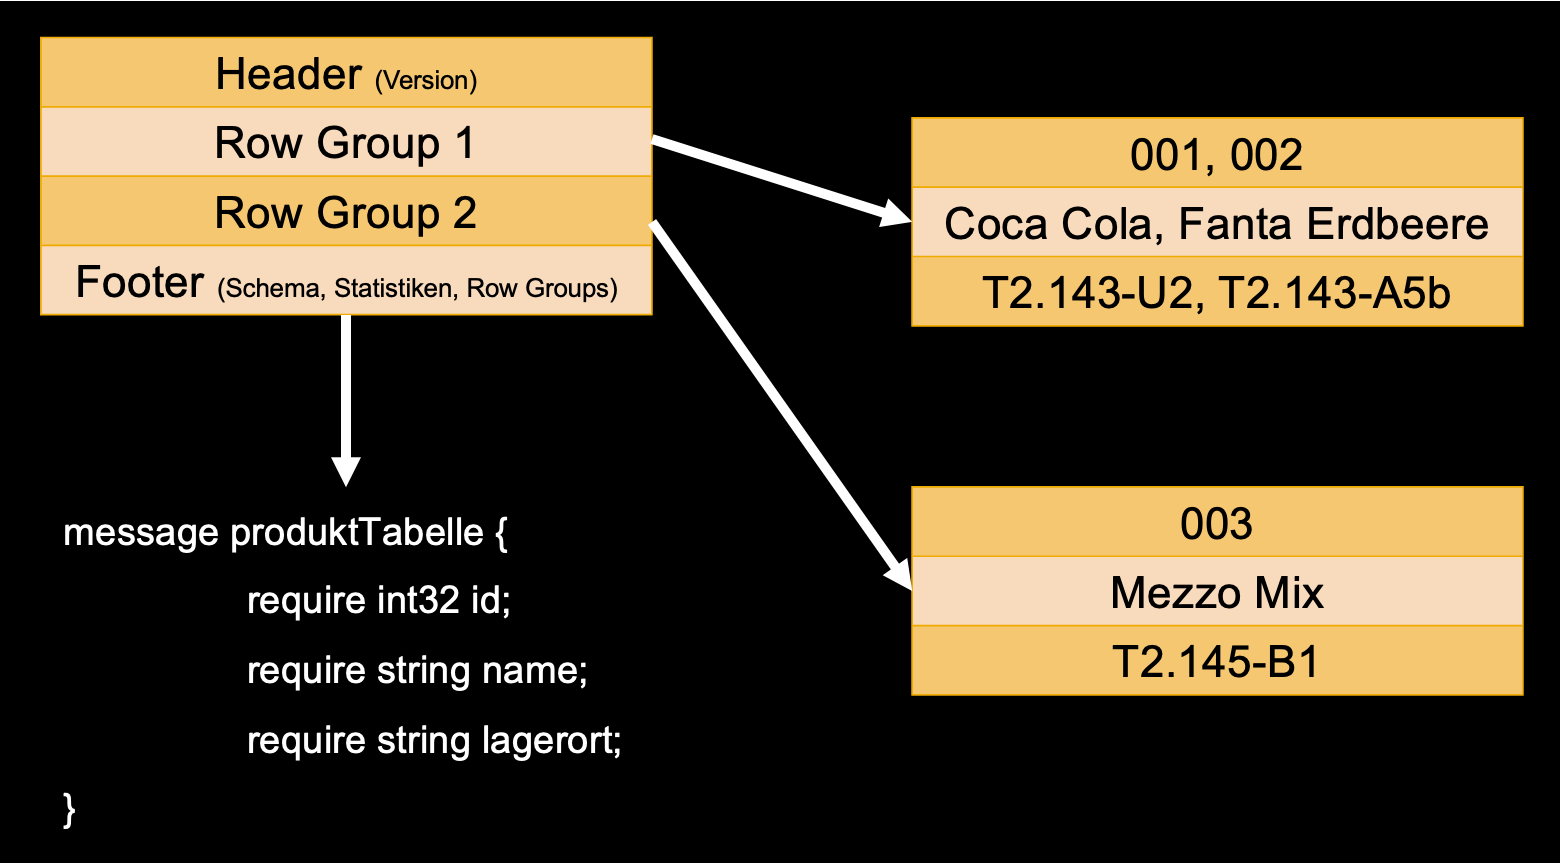
\includegraphics[width=1\textwidth]{Bilder/Parquet.png} 
	\caption{Aufbau von Parquet}
	\label{fig:Parquet}
\end{figure}
\clearpage
\begin{figure}[ht]
	\centering
	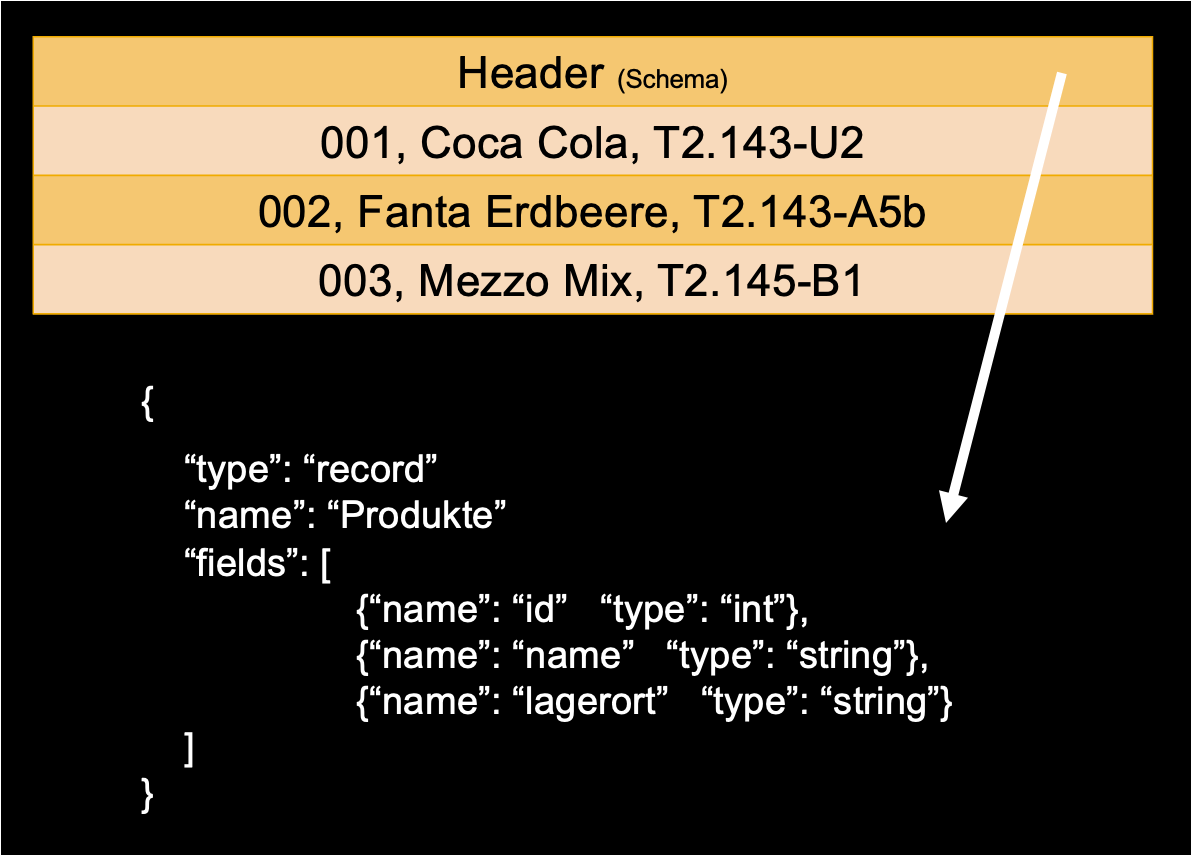
\includegraphics[width=1\textwidth]{Bilder/Avro.png} 
	\caption{Aufbau von Avro}
	\label{fig:Avro}
\end{figure}
\clearpage
\begin{figure}[ht]
	\centering
	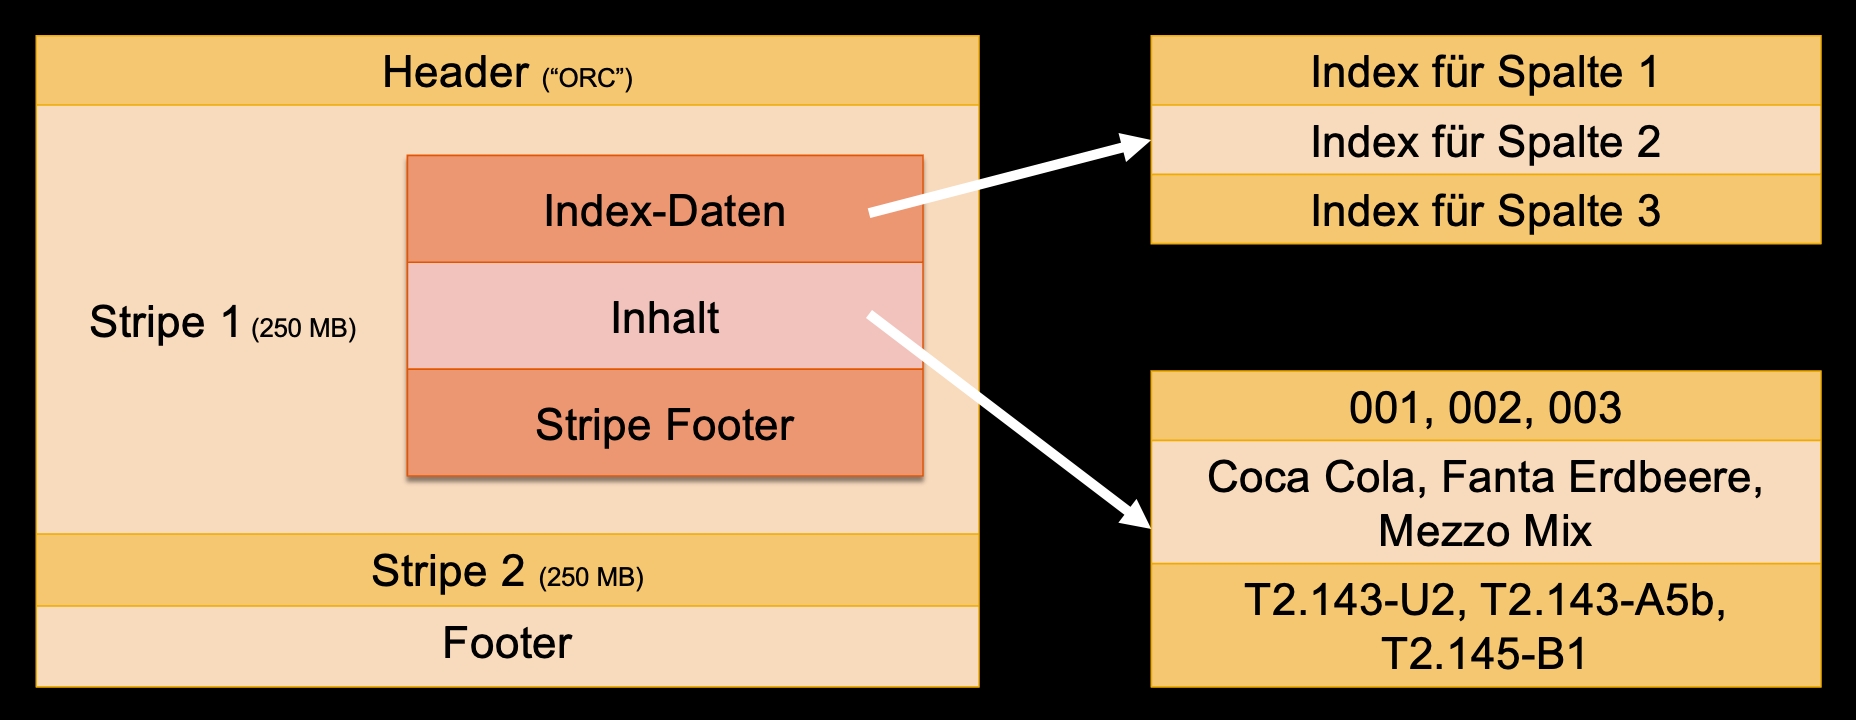
\includegraphics[width=1\textwidth]{Bilder/ORC.png} 
	\caption{Aufbau von ORC}
	\label{fig:ORC}
\end{figure}
\clearpage
\chapter{Vergleiche}
\begin{figure}[ht]
	\centering
	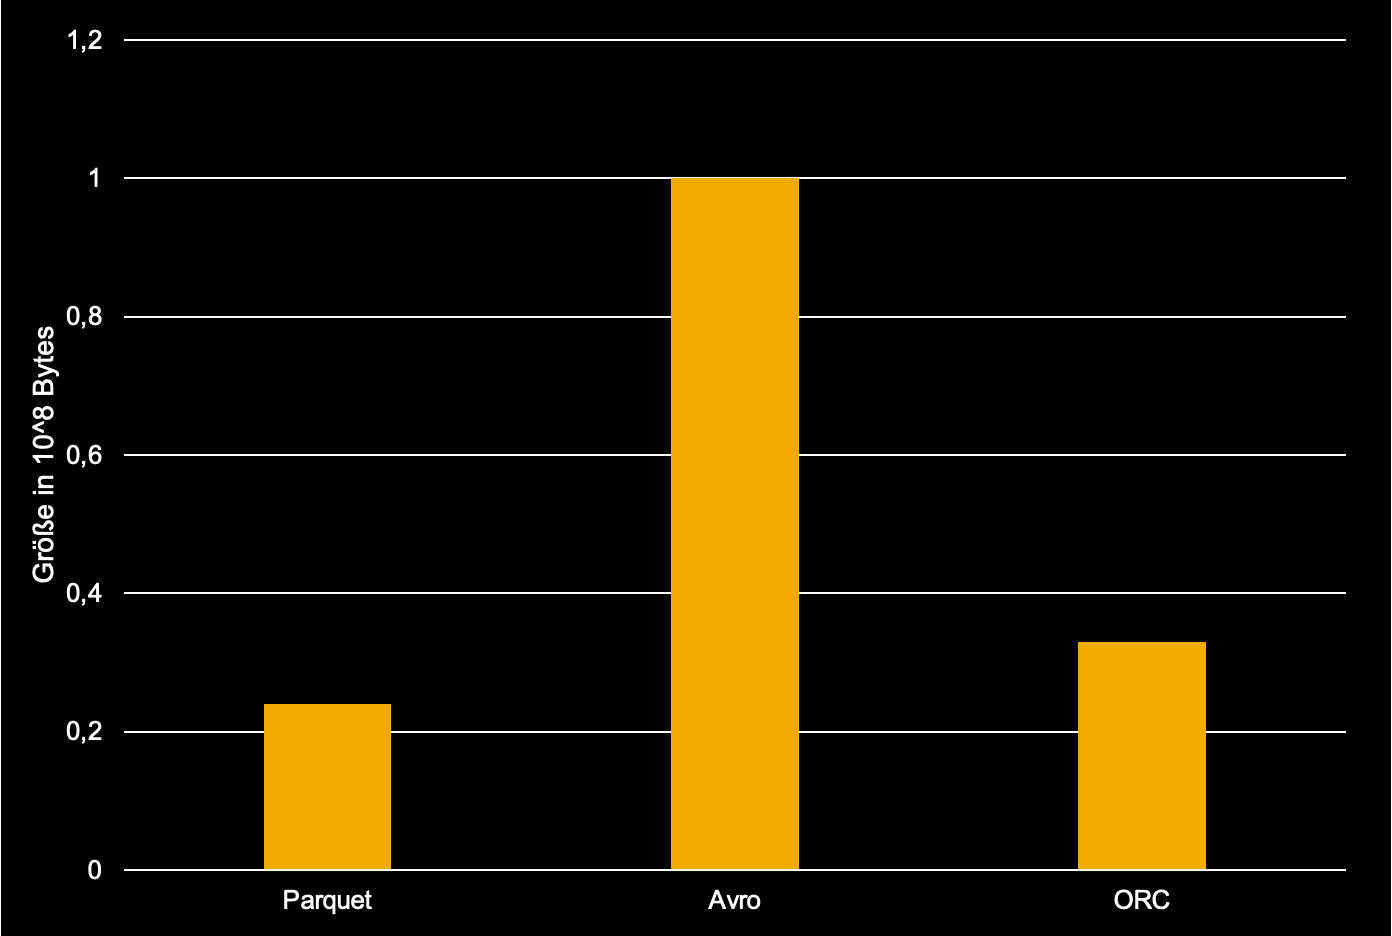
\includegraphics[width=1\textwidth]{Bilder/Speicher.png} 
	\caption{Speicherplatz}
	\label{fig:Speicherplatz}
\end{figure}
\clearpage
\begin{figure}[ht]
	\centering
	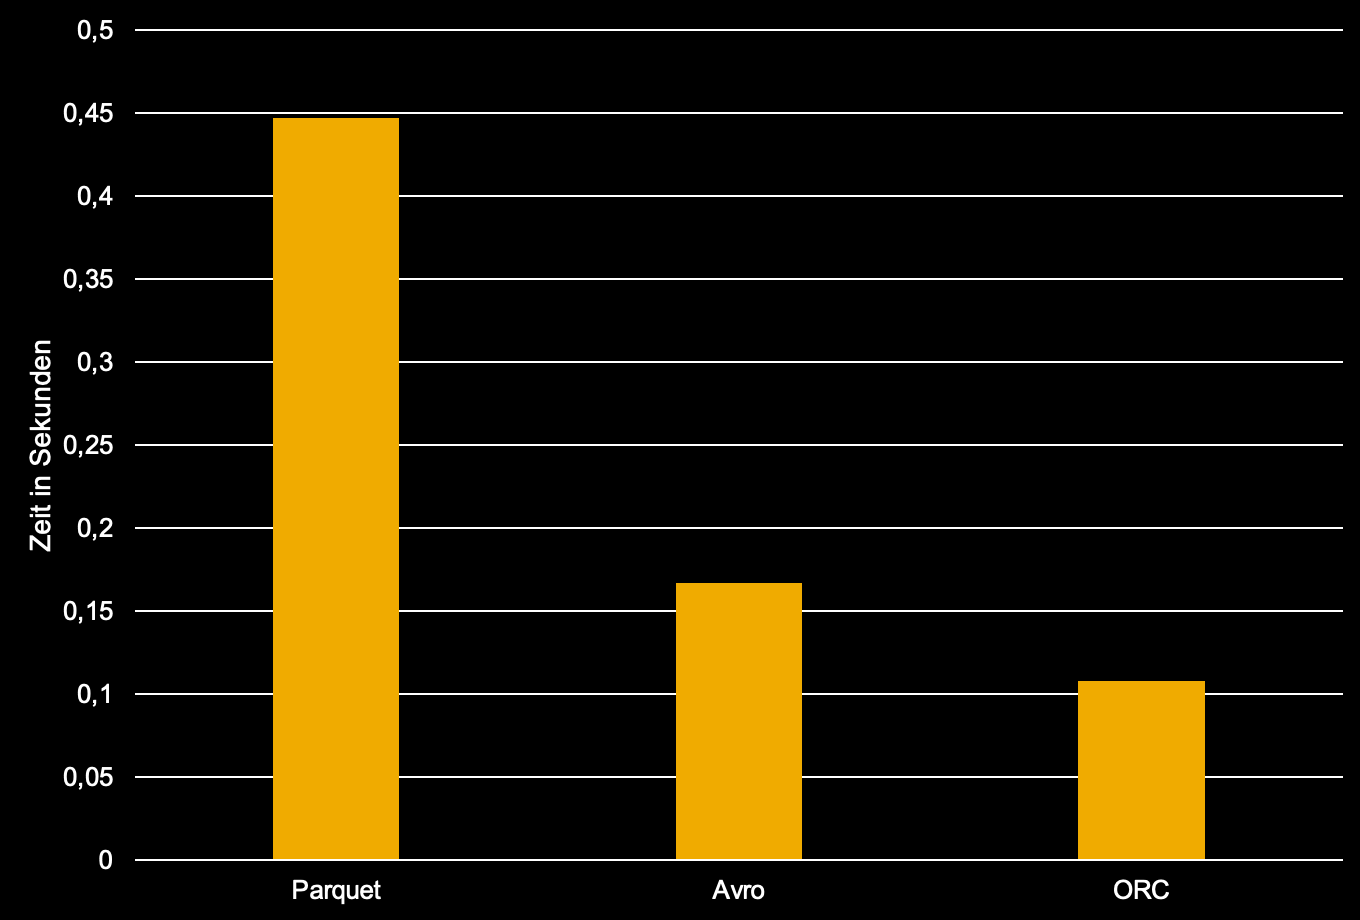
\includegraphics[width=1\textwidth]{Bilder/Lesezugriff.png} 
	\caption{Lesezugriff der gesamten Daten}
	\label{fig:Lesezugriff}
\end{figure}
\clearpage
\begin{figure}[ht]
	\centering
	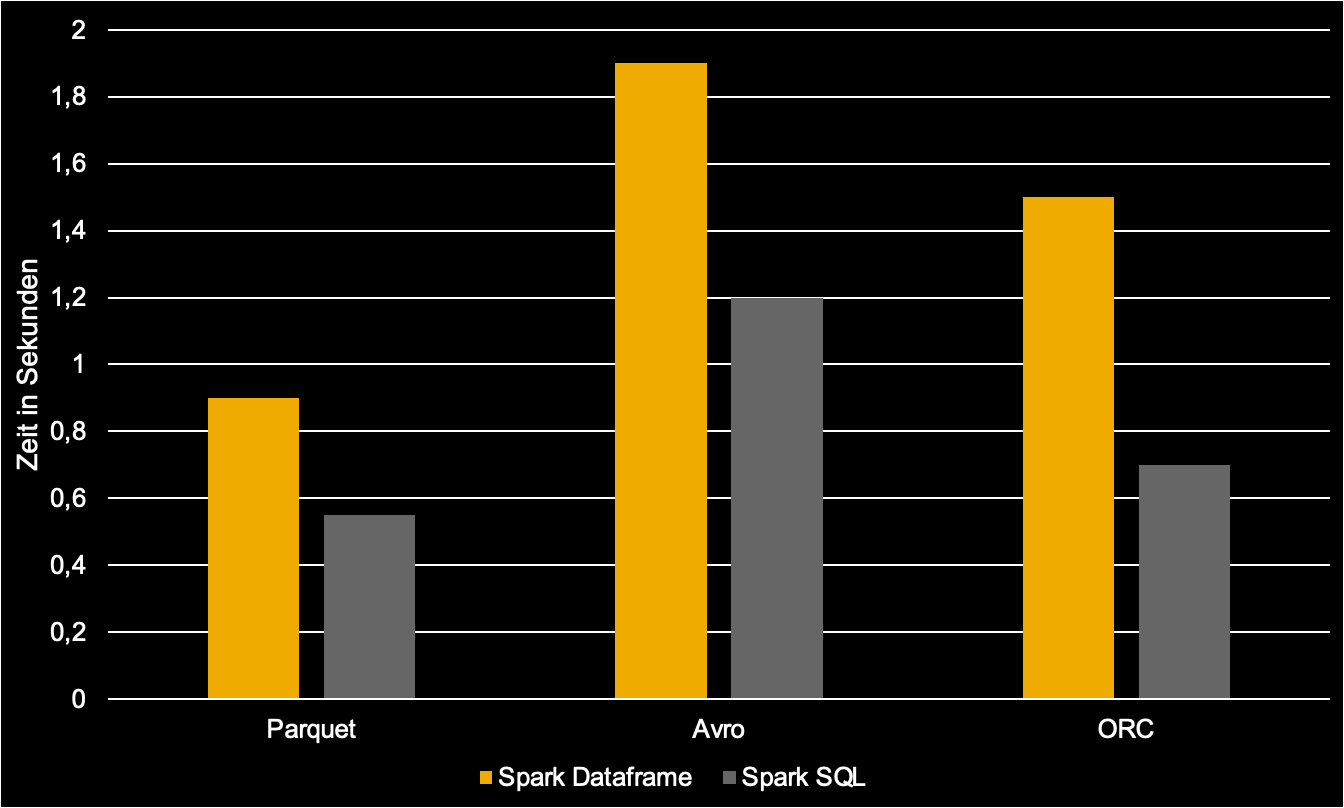
\includegraphics[width=1\textwidth]{Bilder/Zufall.png} 
	\caption{Zufällige Auswahl}
	\label{fig:Zufall}
\end{figure}
\clearpage
\begin{figure}[ht]
	\centering
	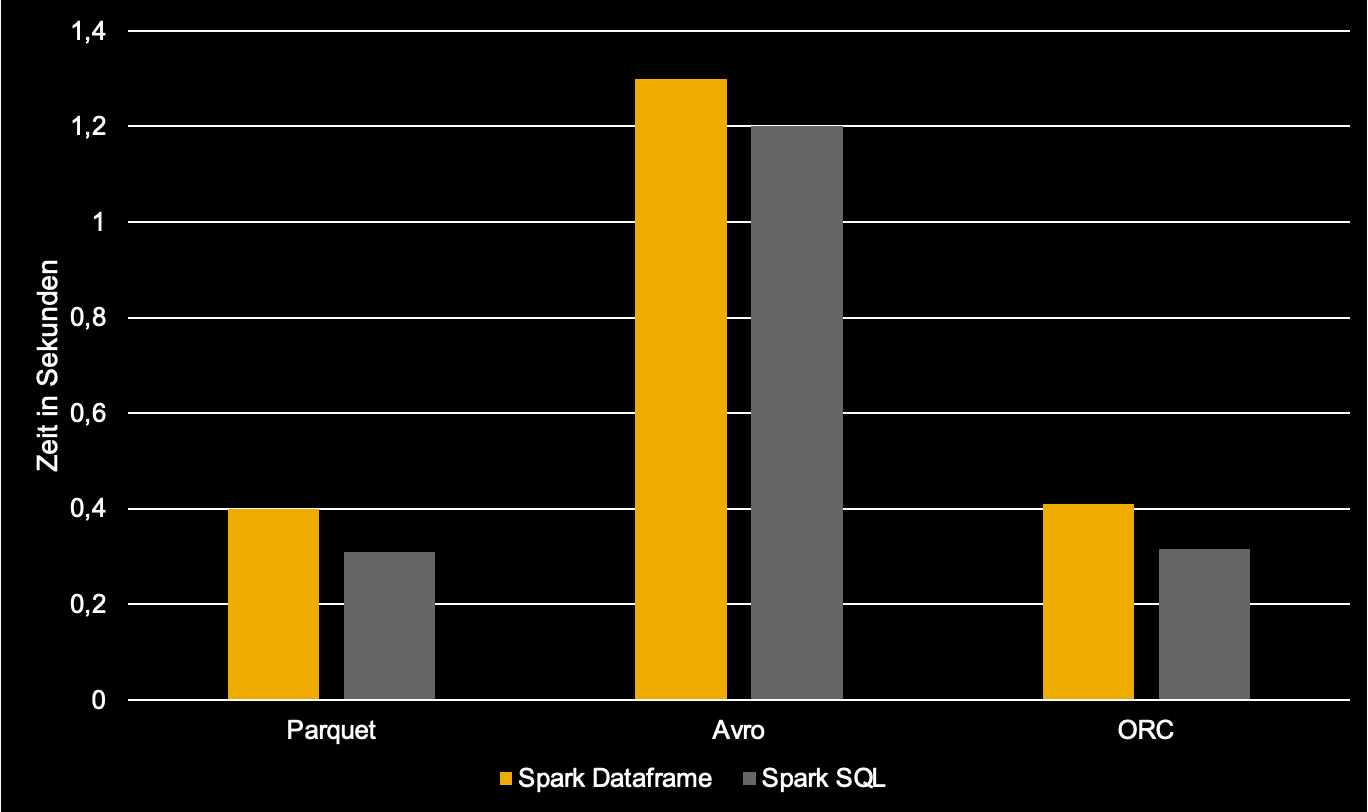
\includegraphics[width=1\textwidth]{Bilder/Aggregation.png} 
	\caption{Aggregation}
	\label{fig:Aggregation}
\end{figure}
\clearpage
\begin{figure}[ht]
	\centering
	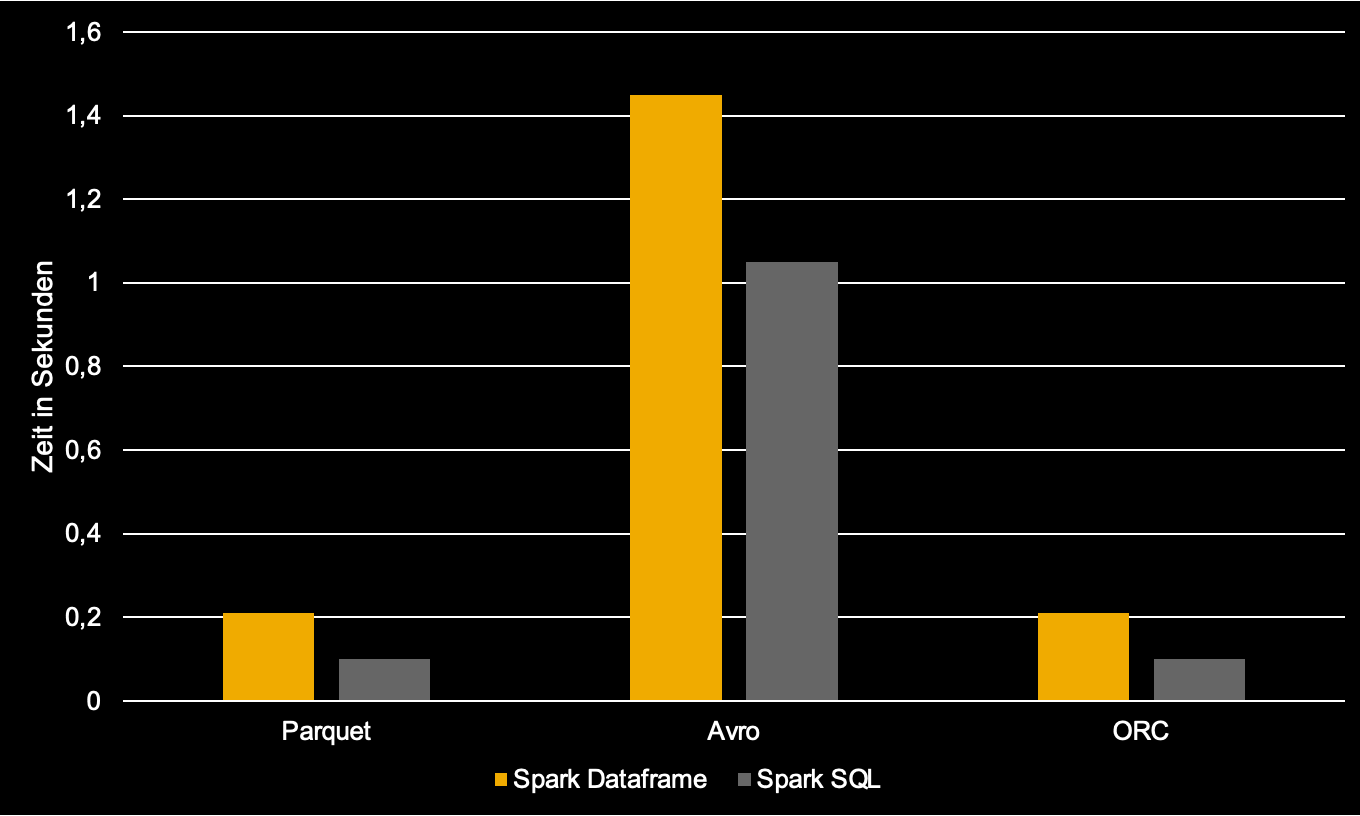
\includegraphics[width=1\textwidth]{Bilder/Summierung.png} 
	\caption{Summierung}
	\label{fig:Summierungen}
\end{figure}
\clearpage
\begin{figure}[ht]
	\centering
	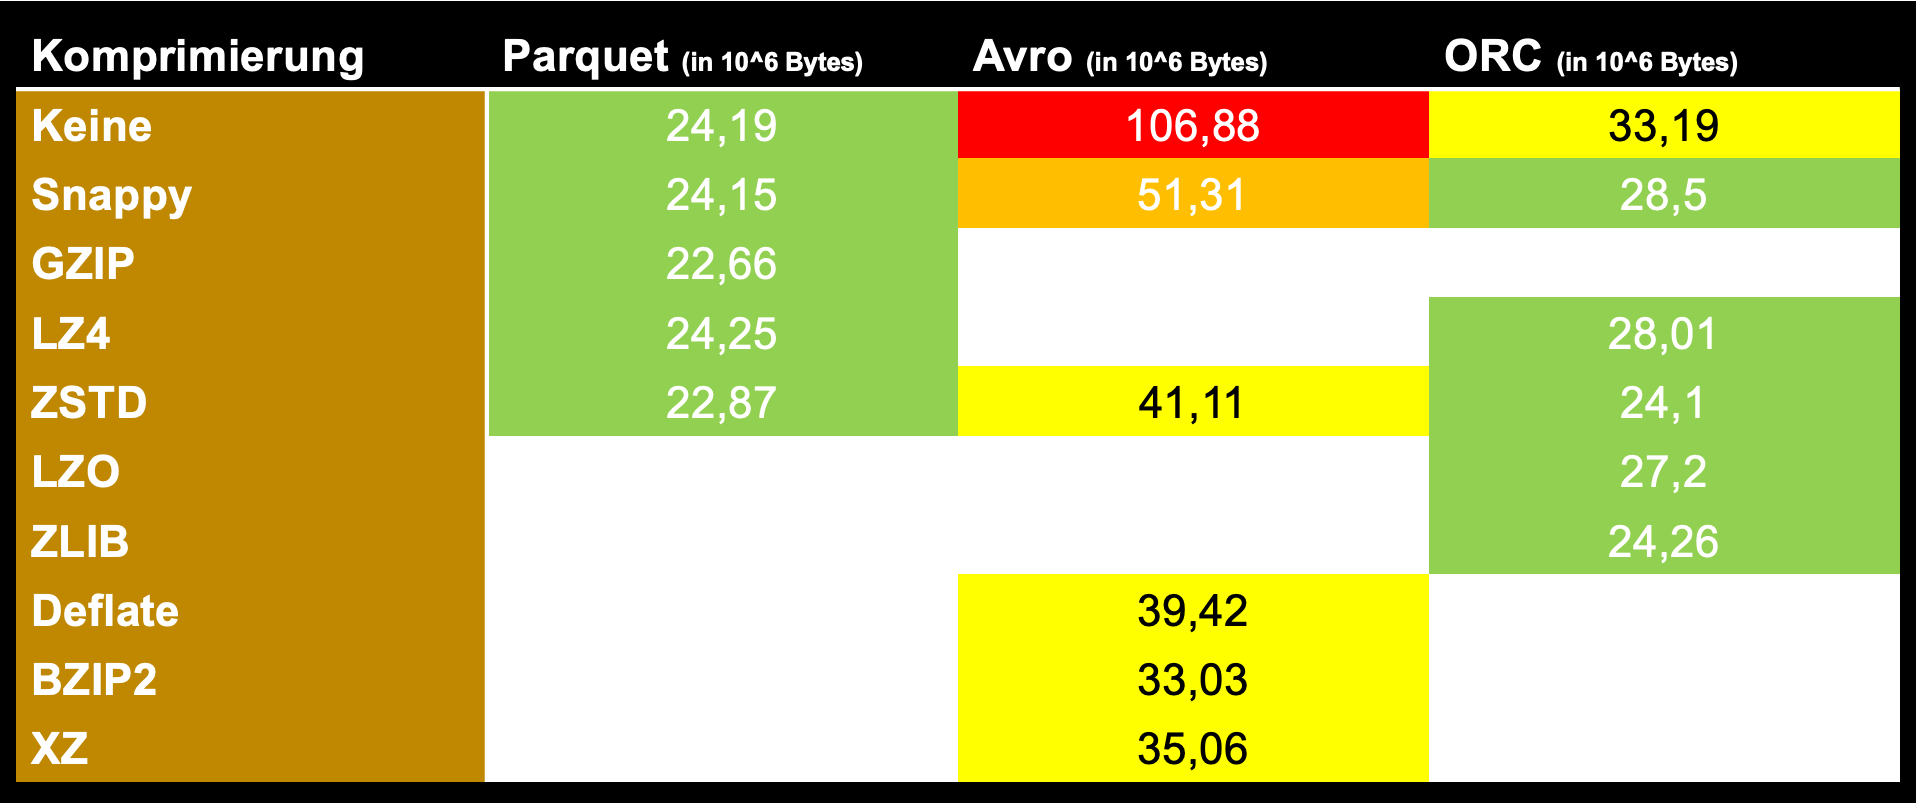
\includegraphics[width=1\textwidth]{Bilder/Komprimierung.png} 
	\caption{Komprimierung}
	\label{fig:Komprimierung}
\end{figure}
\clearpage
\chapter{Code}
\lstinputlisting[
    language=JavaScript,
	label=code:Parquet,    % Label; genutzt für Referenzen auf dieses Code-Beispiel
	caption=Parquet,
	captionpos=b,               % Position, an der die Caption angezeigt wird t(op) oder b(ottom)
	firstline=1,                % Zeilennummer im Dokument welche als erste angezeigt wird
	lastline=2              % Letzte Zeile welche ins LaTeX Dokument übernommen wird
]{Quellcode/code.js}
\lstinputlisting[
    language=JavaScript,
	label=code:Avro,    % Label; genutzt für Referenzen auf dieses Code-Beispiel
	caption=Avro,
	captionpos=b,               % Position, an der die Caption angezeigt wird t(op) oder b(ottom)
	firstline=4,                % Zeilennummer im Dokument welche als erste angezeigt wird
	lastline=9              % Letzte Zeile welche ins LaTeX Dokument übernommen wird
]{Quellcode/code.js}
\lstinputlisting[
    language=JavaScript,
	label=code:ORC,    % Label; genutzt für Referenzen auf dieses Code-Beispiel
	caption=ORC,
	captionpos=b,               % Position, an der die Caption angezeigt wird t(op) oder b(ottom)
	firstline=11,                % Zeilennummer im Dokument welche als erste angezeigt wird
	lastline=15              % Letzte Zeile welche ins LaTeX Dokument übernommen wird
]{Quellcode/code.js}
\lstinputlisting[
    language=JavaScript,
	label=code:XML,    % Label; genutzt für Referenzen auf dieses Code-Beispiel
	caption=XML,
	captionpos=b,               % Position, an der die Caption angezeigt wird t(op) oder b(ottom)
	firstline=41,                % Zeilennummer im Dokument welche als erste angezeigt wird
	lastline=55              % Letzte Zeile welche ins LaTeX Dokument übernommen wird
]{Quellcode/code.js}
\lstinputlisting[
    language=JavaScript,
	label=code:JSON,    % Label; genutzt für Referenzen auf dieses Code-Beispiel
	caption=JSON,
	captionpos=b,               % Position, an der die Caption angezeigt wird t(op) oder b(ottom)
	firstline=21,                % Zeilennummer im Dokument welche als erste angezeigt wird
	lastline=39              % Letzte Zeile welche ins LaTeX Dokument übernommen wird
]{Quellcode/code.js}
\lstinputlisting[
    language=JavaScript,
	label=code:CSV,    % Label; genutzt für Referenzen auf dieses Code-Beispiel
	caption=CSV,
	captionpos=b,               % Position, an der die Caption angezeigt wird t(op) oder b(ottom)
	firstline=17,                % Zeilennummer im Dokument welche als erste angezeigt wird
	lastline=19              % Letzte Zeile welche ins LaTeX Dokument übernommen wird
]{Quellcode/code.js}
\clearpage
\chapter{Datengrundlage}
\begin{figure}[ht]
	\centering
	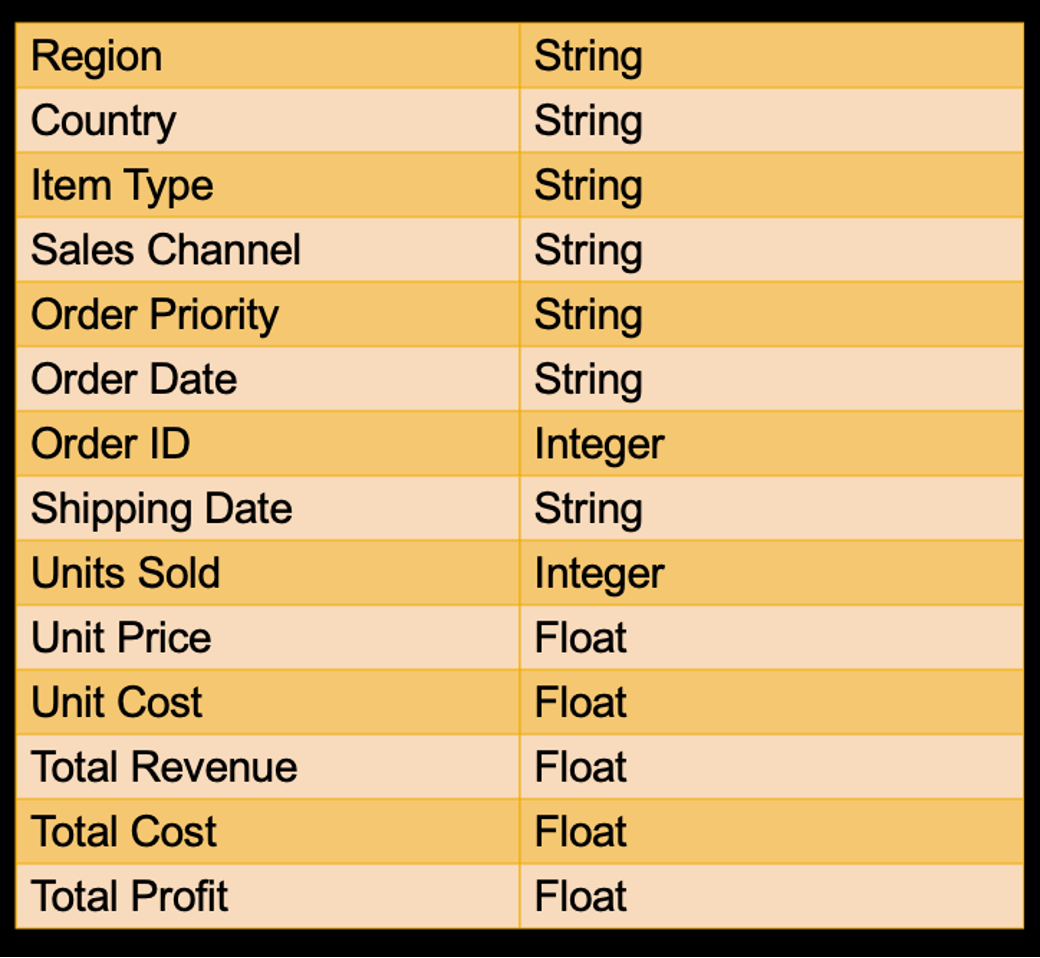
\includegraphics[width=1\textwidth]{Bilder/Daten.png} 
	\caption{Aufbau der Datengrundlage}
	\label{fig:Daten}
\end{figure}

%\clearpage
%\pagenumbering{Roman}  % römische Seitenzahlen für Anhang

\newpage
\end{document}
